\chapter{Fazit}
\label{chap:Fazit}
Ziel dieser Arbeit war es, die Gemeinsamkeiten und Unterschiede zwischen SOA und Microservices herauszuarbeiten. Dazu wurden die Vor- und Nachteile der beiden Paradigmen hinsichtlich Prozessisolierung, Skalierung, Deployment, Wartbarkeit (Korrigierbarkeit, Erweiterbarkeit, Anpassbarkeit, Verbesserung), Entwicklung/Testbarkeit und die Bindung an Technologiestacks herausgearbeitet und anschließend verglichen werden.
\\\\
Nach der Analyse und dem Vergleich der beiden Paradigmen, kann man sagen, dass die Herangehensweise beider Architekturmodelle auf unterschiedlichen Ebenen arbeiten, jedoch das gleiche Ziel verfolgen. Beide Ansätze sollen das Umsetzten neuer Anforderungen vereinfachen.

Bei einem Microservice-System wird dies erreicht, in dem Anwendungen in kleinere Dienste aufgeteilt werden, wodurch die Entwicklung vereinfacht werden soll. Durch die Aufteilung können unterschiedliche Teams an neuen Funktionen arbeiten und deployen, ohne unbedingt auf andere Teams warten zu müssen.

SOA verfolgt hingegen das Ziel, die gesamte Unternehmens-IT zu vereinheitlichen und in einzelne Services aufzuteilen. Dabei wird eine Abstraktionsschicht über den vorhandenen Services eingeführt, um diese neu zu kombinieren. Damit soll erreicht werden, dass eine flexible Integration der vorhandenen Anwendungen möglich ist und nur die Informationen dargestellt und verarbeitet werden, welche wirklich benötigt werden.
\\\\
SOA und Microservices schließen sich nicht gegenseitig aus. Microservice-Systeme können Teil eines SOA-Systems sein und ihre Aufgaben in diesen einbinden. Dabei wird ein Microservice-System wie eine vollständige Anwendung behandelt. Der  Unterschied ist jedoch, dass meistens deutlich mehr Schnittstellen zur Verfügung gestellt werden können, aufgrund der internen Struktur.
\begin{figure}[htb]
    \centering 
    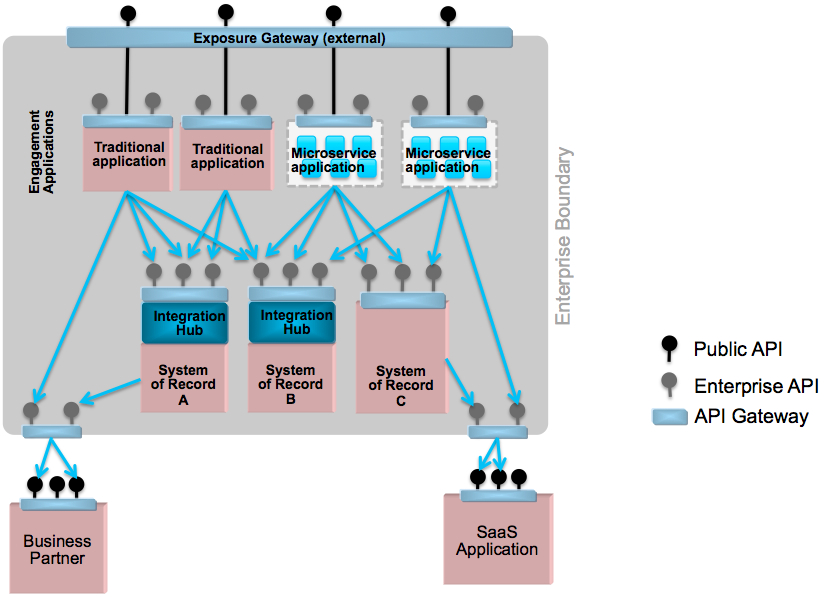
\includegraphics[width=\textwidth]{content/images/figure8}\
    \quelle\url{https://www.ibm.com/developerworks/websphere/library/techarticles/1601_clark-trs/1601_clark.html}
    \caption{Microservice, SOA und APIs Kombiniert}
    \label{fig:MicroservicesSOAAndAPIsCombined} 
\end{figure}

Möchte man eine Service-orientierte Architektur einsetzten, muss zunächst einmal die Frage gestellt werden, welchen Zweck damit erfüllt werden soll und welches Einsatzgebiet abgedeckt werden soll. Während mit Microservices die Entwicklung vereinfacht werden soll, wird mit SOA versucht die vorhandenen Unternehmensanwendungen zu strukturieren.
\\\\
Außerdem darf der Aufwand bei der Einführung eines neuen Architekturmusters nicht unterschätzt werden. Möchte ein Unternehmen beispielsweise SOA einführen, müssen alle Systeme im Unternehmen so angepasst werden, dass sie als Dienste verwendet werden können. Die Einführung von SOA betrifft somit das gesamte Unternehmen. Dabei ist das \textit{Gesetzt von Conway} zu beachten, wodurch häufig die Abteilungen eines Unternehmens neu strukturiert werden müssen, um SOA einzuführen. 

Bei der Einführung von einem Microservice-System betrifft diese Entscheidung zunächst einmal, nur ein Projekt, welches jedoch der Anfang von weiteren Microservice-Systemen sein kann.
\\\\
Zudem sollte nicht nur die Fragen nach dem Zweck gestellt werden, sondern auch nach den Einsatzmöglichkeiten. Wird ein System benötigt, welches einfach zu skalieren ist oder ein System, bei dem die Anwendungen besser strukturiert sind. Während in einem Microservice-System deutlich einfacher Skaliert werden kann, als in einem SOA-System, werden durch die Schnittstellen sehr viele Informationen bereitgestellt. Bei einem SOA-System hingegen wird dafür gesorgt, dass die Informationen gefiltert und aufbereitet werden, sodass der Nutzer nur die Informationen bekommt. Durch den Aufbau beider Muster, ist es jedoch möglich, durch das hinzufügen oder ändern von Services, neue Geschäftsprozesse schneller zu etablieren.
\\\\
Ein wichtiger Punkt der Entscheidung ist die Wartbarkeit, solcher Systeme. Die Wartung muss ein aktiver Prozess in allen Stadien sein. Dies betrifft die Entwicklung, das Testen, das Deployment und die Skalierung. Zudem ist die Bindung an Technologie Stacks ein wichtiges Thema. Möchte ein Unternehmen immer die neuste Technologie einsetzten, dürfte dies mit einem SOA-System schwieriger sein, als mit meinem Microservice-System.
\\\\
Abschließend kann man sagen, dass beide Paradigmen, zwar unterschiedliche Ansätze besitzen, jedoch das gleiche Ziel verfolgen: Das schnellere und einfachere Umsetzen von neuen Anforderungen. Dabei können beide Ansätze, aufgrund der unterschiedlichen Einsatzgebiete, gleichzeitig in einem Unternehmen eingesetzt werden. Bei der Einführung einer Service-orientierten Architektur, sollte gründlich analysiert werden, welche Eigenschaften das einzusetzende Paradigma erfüllen muss und wie viel Aufwand die Umsetzung bedeutet.

\section{Ausblick}
\label{sec:Ausblick}
In der Bachelorarbeit soll eine Anwendung, für die Zusammenarbeit, beispielhaft mit dem Microservice Paradigma erstellt werden. Anhand diesem beispielhaften System soll untersucht werden, welche Voraussetzungen gegeben sein müssen, um ein Microservice-System zu betreiben und welche Werkzeuge eingesetzt werden müssen, um ein Microservice-System aufzubauen, bzw. zu verwenden und zu verwalten. Konkret soll Untersucht werden, wie genau ein Microservice deployed und skaliert werden kann. Zudem soll untersucht werden wie Microservices in solch einem System gefunden und verwendet werden können. außerdem soll untersucht werden, wie die Benutzerverwaltung und die Authentifizierung in solch einem System funktioniert. Konkret soll untersucht werden, wie Benutzerberechtigungen verwaltet und abgefragt werden können, welche unterschiedlichen Ansätze dafür existieren und welche Vor- und Nachteile die jeweiligen Ansätze besitzen. Zusätzlich soll untersucht werden, wie das Monitoring in solch einem System funktioniert.